%----------createAttribute----------------------------------------
\op
{createAttribute}
{creates a new attribute}
{createAttribute(Class selectedEObject, String nameValue)}
{The class providing the container for the newly created attribute.}
{
\begin{itemize}
 \item nameValue/newName: The name of the newly created attribute
 \item idValue/idName: The id of the newly created attribute
\end{itemize}
}
{There is no attribute in the same context whose name equals the parameter-value
of 'newName' (see
\ref{subsec:checkOtherNames})} 
{Only the name and the id will be set via input data. Visibility, isStatic,
isFinal and isReadOnly will be set with a default value as defined with the
diagram editor in the image below.} \begin{figure}[H]
  \centering
  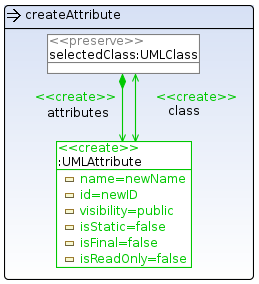
\includegraphics[width=0.4\textwidth]{pics/createAttributeInClass.png}    
  \caption{createAttribute}
  \label{createAttribute}  
\end{figure}
%----------deleteAttribute----------------------------------------
\op
{deleteAttribute}
{Deletes an attribute}
{deleteAttribute(Attribute selectedEObject)}
{The attribute which should be deleted} {-}
{-}
{For a better readability this is a simplified version of the
'deleteAttribute'-transformation and will only cover cases where the attribute
has no no references to other elements. Such a complex
transformation rule exits but won't be listed here.}
\begin{figure}[H]
  \centering
  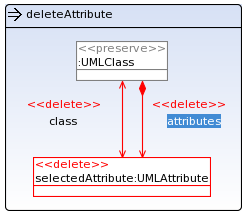
\includegraphics[width=0.4\textwidth]{pics/deleteAttribute_emptyAndUnreferenced.png}    
  \caption{deleteAttribute}
  \label{deleteAttribute}  
\end{figure}
%----------editAttributeName----------------------------------------
\op
{editAttributeName}
{edits the name of an attribute}
{editAttributeName(Attribute selectedEObject, String nameValue)}
{The attribute whose name should be renamed.}
{
\begin{itemize}
 \item nameValue/newName: The new name
\end{itemize}
}
{There is no attribute in the same class whose name equals the parameter-value of
'newName' (see
\ref{subsec:checkOtherNames})}
{The \textless\textless create\textgreater\textgreater  -symbol in the image
means that even if the attribute exists its value will be overwritten.
'newName' is the placeholder for the input name.}
\begin{figure}[H]
  \centering
  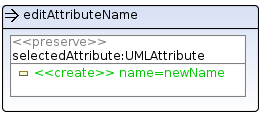
\includegraphics[width=0.4\textwidth]{pics/editAttributeName.png}    
  \caption{editAttributeName}
  \label{editAttributeName}  
\end{figure}
%----------editAttributeIsReadOnly----------------------------------------
\op
{editAttributeIsReadOnly}
{edits the isReadOnly-value of an attribute}
{editAttributeIsReadOnly(Attribute selectedEObject, boolean booleanValue)}
{The attribute whose isReadOnly-value should be edited.}
{
\begin{itemize}
 \item booleanValue/bool: The new isReadOnly-value
\end{itemize}
}
{-}
{The \textless\textless create\textgreater\textgreater  -symbol in the image
means that even if the attribute exists its value will be overwritten.
'bool' is the placeholder for the input boolean value.}
\begin{figure}[H]
  \centering
  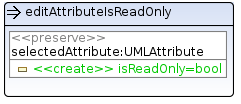
\includegraphics[width=0.4\textwidth]{pics/editAttributeIsReadOnly.png}    
  \caption{editAttributeIsReadOnly}
  \label{editAttributeIsReadOnly}  
\end{figure}
%----------editAttributeIsStatic----------------------------------------
\op
{editAttributeIsStatic}
{edits the isStatic-value of an attribute}
{editAttributeIsStatic(Attribute selectedEObject, boolean booleanValue)}
{The attribute whose isStatic-value should be edited.}
{
\begin{itemize}
 \item booleanValue/bool: The new isStatic-value
\end{itemize}
}
{-}
{The \textless\textless create\textgreater\textgreater  -symbol in the image
means that even if the attribute exists its value will be overwritten.
'bool' is the placeholder for the input boolean value.}
\begin{figure}[H]
  \centering
  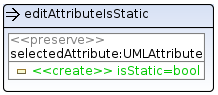
\includegraphics[width=0.4\textwidth]{pics/editAttributeIsStatic.png}    
  \caption{editAttributeIsStatic}
  \label{editAttributeIsStatic}  
\end{figure}
%----------editAttributeIsFinal----------------------------------------
\op
{editAttributeIsFinal}
{edits the isFinal-value of an attribute}
{editAttributeIsFinal(Attribute selectedEObject, boolean booleanValue)}
{The attribute whose isFinal-value should be edited.}
{
\begin{itemize}
 \item booleanValue/bool: The new isFinal-value
\end{itemize}
}
{-}
{The \textless\textless create\textgreater\textgreater  -symbol in the image
means that even if the attribute exists its value will be overwritten.
'bool' is the placeholder for the input boolean value.}
\begin{figure}[H]
  \centering
  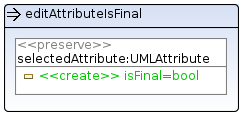
\includegraphics[width=0.4\textwidth]{pics/editAttributeIsFinal.png}    
  \caption{editAttributeIsFinal}
  \label{editAttributeIsFinal}  
\end{figure}
%----------editAttributeVisibility----------------------------------------
\op
{editAttributeVisibility}
{edits the visibility of an attribute}
{editAttributeVisibility(Attribute selectedEObject, Visibility visibilityValue)}
{The attribute whose visibility should be edited.}
{
\begin{itemize}
 \item visibilityValue/visibility: The new visiblility
\end{itemize}
}
{-}
{The \textless\textless create\textgreater\textgreater  -symbol in the image
means that even if the attribute exists its value will be overwritten.
'visibility' is the placeholder for the input visibility value.}
\begin{figure}[H]
  \centering
  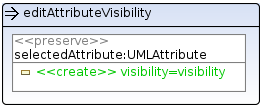
\includegraphics[width=0.4\textwidth]{pics/editAttributeVisibility.png}    
  \caption{editAttributeVisibility}
  \label{editAttributeVisibility}  
\end{figure}
%----------editAttributeTypeFromClassToClass----------------------------------------
\op
{editAttributeTypeFromClassToClass}
{edits the type of an attribute from a class to another}
{editAttributeTypeFromClassToClass(Attribute selectedEObject, Class typeValue)}
{The attribute whose type should be edited.}
{
\begin{itemize}
 \item typeValue/newType: The new type
\end{itemize}
}
{-}
{Only references will change.}
\begin{figure}[H]
  \centering
  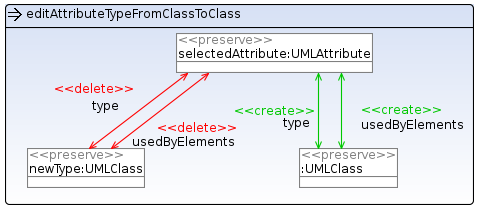
\includegraphics[width=0.7\textwidth]{pics/editAttributeTypeFromClassToClass.png}    
  \caption{editAttributeTypeFromClassToClass}
  \label{editAttributeTypeFromClassToClass}  
\end{figure}
%----------editAttributeTypeFromClassToPrimitive----------------------------------------
\op
{editAttributeTypeFromClassToPrimitive}
{edits the type of an attribute from a class to a primitiveType}
{editAttributeTypeFromClassToPrimitive(Attribute selectedEObject, PrimitiveType typeValue)}
{The attribute whose type should be edited.}
{
\begin{itemize}
 \item typeValue/newType: The new type
\end{itemize}
}
{-}
{Only references will change.}
\begin{figure}[H]
  \centering
  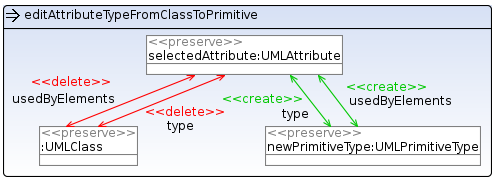
\includegraphics[width=0.7\textwidth]{pics/editAttributeTypeFromClassToPrimitive.png}    
  \caption{editAttributeTypeFromClassToPrimitive}
  \label{editAttributeTypeFromClassToPrimitive}  
\end{figure}
%----------editAttributeTypeFromPrimitiveToClass----------------------------------------
\op
{editAttributeTypeFromPrimitiveToClass}
{edits the type of an attribute from a primitiveType to a class}
{editAttributeTypeFromPrimitiveToClass(Attribute selectedEObject, Class typeValue)}
{The attribute whose type should be edited.}
{
\begin{itemize}
 \item typeValue/newType: The new type
\end{itemize}
}
{-}
{Only references will change.}
\begin{figure}[H]
  \centering
  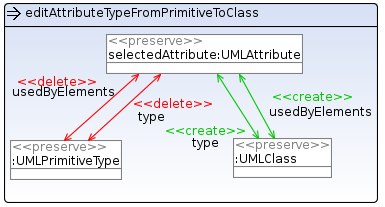
\includegraphics[width=0.60\textwidth]{pics/editAttributeTypeFromPrimitiveToClass.png}    
  \caption{editAttributeTypeFromPrimitiveToClass}
  \label{editAttributeTypeFromPrimitiveToClass}  
\end{figure}
%----------editAttributeTypeFromPrimitiveToPrimitive----------------------------------------
\op
{editAttributeTypeFromPrimitiveToPrimitive}
{edits the type of an attribute from a primitiveType to a primitiveType}
{editAttributeTypeFromPrimitiveToPrimitive(Attribute selectedEObject, PrimitiveType typeValue)}
{The attribute whose type should be edited.}
{
\begin{itemize}
 \item typeValue/newType: The new type
\end{itemize}
}
{-}
{Only references will change.}
\begin{figure}[H]
  \centering
  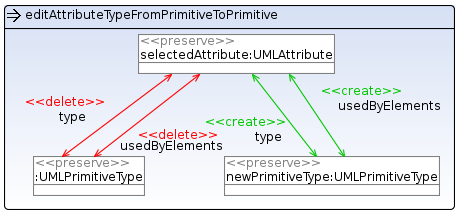
\includegraphics[width=0.7\textwidth]{pics/editAttributeTypeFromPrimitiveToPrimitive.png}    
  \caption{editAttributeTypeFromPrimitiveToPrimitive}
  \label{editAttributeTypeFromPrimitiveToPrimitive}  
\end{figure}
%----------moveAttributeBetweenClasses----------------------------------------
\op
{moveAttribute}
{moves an attribute from a class to another class}
{moveAttributeBetweenClasses(Attribute selectedEObject, class tgt)}
{The attribute which should be moved.}
{
\begin{itemize}
 \item tgt/tgt[moveAttribute]: the target class
\end{itemize}
}
{There is no attribute with the same name in the target context (see
\ref{subsec:checkOtherNames})}
{Only references will change.}
\begin{figure}[H]
  \centering
  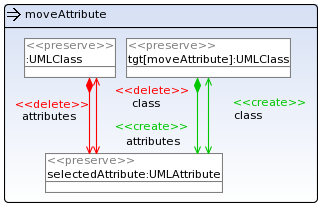
\includegraphics[width=0.5\textwidth]{pics/moveAttribute.png}    
  \caption{moveAttribute}
  \label{moveAttribute}  
\end{figure}